\documentclass[12pt, a4paper]{article}
\usepackage{meu}
\usepackage{booktabs}
\usepackage{siunitx}

\renewcommand{\thefootnote}{\roman{footnote}}
\setlength{\headheight}{15pt}

\begin{document}
\capa%
\tableofcontents%
\listoffigures\cleardoublepage%

\section{Introdução}\label{sec:intro}
O Projeto tem como objetivo a implementação de um sistema para auxiliar turistas em Veneza a chegarem aos diversos museus da cidade,
localizados em diferentes ilhas.

Implementado inteiramente em c++20 sem utilização de bibliotecas externas além das bibliotecas padrão do c++20,
podendo assim ser compilado em qualquer sistema operacional que possua o compilador adequado.

Essa linguagem foi escolhida pois além de possuir abstrações alto nível com o uso de classes,
ainda é extremamente eficiente ao ser compilada diretamente para para linguagem de máquina.
Além do disso a dupla responsável pelo projeto possui familiaridade com a linguagem.

O sistema é capaz de calcular a rota mais curta entre dois pontos,
utilizando os algoritmos A*, busca em largura e busca em profundidade.

Visando a simplicidade e levar os algoritmos a seus limites de eficiência,
o sistema não implementa uma interface gráfica,
todos os argumentos devem ser passados como argumentos de linha de comando,
ou coletados em tempo de execução, para ver os argumentos para o programa veja a seção~\nameref{sec:executando}.

Uma vez que todos os parâmetros para execução do programa podem ser passados antes que ele inicie,
pode-se fazer uso de scripts para automatizar a execução do programa gerando resultados para diferentes cenários.
Dessa maneira foi implementado um script para testar o desempenho, explicado na seção~\nameref{sec:testes}.

\section{Executando o programa}\label{sec:executando_programa}
\subsection{Requisitos}\label{sec:requisitos}
\begin{itemize}
    \item cmake;
    \item make;
    \item g++;
    \item git (opcional).
\end{itemize}

\subsection{Compilando}\label{sec:compilando}
Antes de realizar a compilação é necessário definir o nível de mensagens que serão exibidas durante a execução do programa.

Para isso basta definir a expressão \texttt{DEFAULT\_LOG\_LEVEL}, no arquivo\\\texttt{logger.hpp},
para um dos valores definidos no enum \texttt{LogLevel}:
\begin{lstlisting}[caption={Enum LogLevel}, label={lst:log}]
    enum LogLevel { DEBUG, INFO, WARNING, ERROR, FATAL };
\end{lstlisting}

Caso o valor seja definido como:
\begin{itemize}
    \item\textbf{DEBUG}: Todas as mensagens serão exibidas, tais como objeto construído, objeto destruído, tempos de execução de funções intermediárias, etc.
    \item\textbf{INFO}: Exibe mensagens ``Modo iterativo'' dos algoritmos, como a ilha que está sendo visitada, entre outras.
    \item\textbf{WARNING}: Exibe mensagens de aviso como quando um arquivo não é encontrado.
    \item\textbf{ERROR}: Exibe mensagens de erro na qual ainda é possível continuar a execução do programa.
    \item\textbf{FATAL}: Exibe apenas mensagens de erro que impossibilitam a execução do programa, nível que menos exibe mensagens.
\end{itemize}

Uma vez definido qual o nível de mensagens que serão exibidas, basta compilar o programa com os comandos:
\begin{itemize}
    \item Entrar na pasta build: \texttt{cd build}
    \item Configurar o projeto: \texttt{cmake .}
    \item Compilar o projeto: \texttt{make}
\end{itemize}

\subsection{Executando}\label{sec:executando}
Para executar o programa basta executar o arquivo

\texttt{Graph\_Search\_Algorithms\_1.0.0} gerado na pasta build.

Caso nada seja passado como argumento, o programa irá coletar os argumentos em tempo de execução,
sendo eles:
\begin{enumerate}
    \item O caminho para o arquivo de entrada;
    \item O caminho para o arquivo de saída contendo o resumo da execução;
    \item O algoritmo a ser utilizado, podendo ser:
    \begin{itemize}
        \item A \( \rightarrow \) A*;
        \item B \( \rightarrow \) \textit{BFS, Breadth First Search} (busca em largura);
        \item D \( \rightarrow \) \textit{DFS, Depth First Search} (busca em profundidade).
    \end{itemize}
\end{enumerate}

Exemplos de execução:
\begin{itemize}
    \item\textbf{Sem argumentos:} \texttt{./Graph\_Search\_Algorithms\_1.0.0}
    \item\textbf{Com argumentos:} \texttt{./Graph\_Search\_Algorithms\_1.0.0\\input\_files/exemplo\_prof.txt output.txt A}
\end{itemize}

\subsection{Saída}\label{sec:saida}
Caso a execução seja bem sucedida, o programa irá gerar um arquivo de saída contendo o resumo da execução,
que deverá ser semelhante ao exemplo abaixo:
\begin{figure}[!h]
    \centering
    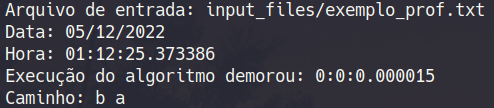
\includegraphics[width=0.8\textwidth]{saida_teste.png}
    \caption{Exemplo de arquivo de saída do programa}
    \label{fig:saida_teste}
\end{figure}


\section{Implementação}\label{sec:impl}
Essa seção visa explicar a implementação do programa,
especificando seus algoritmos e estruturas de dados.

Para mais detalhes da implementação, tais como todas as classes e seus métodos,
pode-se consultar a documentação em \url{https://graph-search-algorithms.pages.dev/}

\subsection{Estruturas de dados}\label{sec:estruturas}
Segue abaixo a descrição das estruturas de dados utilizadas no programa.

\begin{lstlisting}[caption={Estrutura de dados para representar um nó do grafo.}, label={lst:node}]
    enum NodeState { HAS_NONE = 0, HAS_WEIGHT, HAS_HEURISTIC, HAS_BOTH };

    class AdjacencyNode {
    private:
        std::string _id;
        int16_t _weight;
        int16_t _heuristic;
        NodeState _state;
    };
\end{lstlisting}

\begin{lstlisting}[caption={Estrutura de dados para representar o grafo.}, label={lst:graph}]
    class Graph {
    private:
        std::unordered_map<std::string, std::vector<AdjacencyNode>> _nodes;
        std::string _start_node;
        std::string _end_node;
        Algorithms _algorithm;
    };
\end{lstlisting}

Para representação do grafo foi utilizado uma lista de adjacência,
porém ao invés de utilizar um vetor, como normalmente é utilizado,
optou-se por usar um \textit{unordered\_map}, tabela hash, para armazenar os nós do grafo.
Visto que no arquivo de entrada possui nomes de ilhas e não números para identificar os nós,
dessa forma para utilizar um vetor seria necessário um mapeamento entre os nomes e os números,
o que poderia dificultar a implementação.

A estrutura grafo também armazena o identificador do nó inicial e final,
bem como o algoritmo a ser utilizado.
Sendo assim o grafo é o objeto que contém todos os dados necessários para a execução do programa.

\subsection{Algoritmos de busca}\label{sec:algoritmos}
A seguir é apresentado os algoritmos de busca implementados no programa.

\subsubsection{Algoritmo A* (melhor solução)}\label{sec:astar}
Algoritmo de busca ótimo que utiliza uma heurística para encontrar a melhor solução.

Escolhe o próximo nó a ser visitado com base no custo total do caminho, \( g(n) \), até o nó somado com o custo estimado do nó até o nó final, \( h(n) \),
sendo esse custo estimado a heurística do nó. Sendo representado matematicamente por:
\begin{equation}
    f(n) = g(n) + h(n)
\end{equation}

A complexidade de tempo deste algoritmo é \( O(b^d) \), sendo \( b \) a ramificação do grafo e \( d \) a profundidade da solução,
porém caso a possua uma boa heurística a resposta será encontrada em menos iterações. Por esse motivo foi escolhido como melhor solução.

\subsubsection{Busca em profundidade (extra)}\label{sec:bp}
Algoritmo de busca cega não ótimo e completo, devido ao fato de existir um número finito de ilhas (espaço de busca ser finito).

Sempre escolhe o nó mais profundo na árvore de busca para visitar.

A complexidade de tempo deste algoritmo é \( O(b^m) \), sendo \( b \) a ramificação do grafo e \( m \) a profundidade da solução,
e a complexidade de espaço é \( O(bm) \).

\subsubsection{Busca em largura (pior solução)}\label{sec:bl}
Algoritmo de busca cega completo e ótimo, com implementação simples.

Escolhe o próximo nó a ser visitado com base na profundidade do nó,
sendo o nó mais próximo do nó inicial escolhido primeiro.

A complexidade de tempo deste algoritmo é \( O(b^d) \), sendo \( b \) e \( d \) explicados na seção \nameref{sec:astar} a cima.

Pelo fato deste algoritmo gastar mais memória que o algoritmo de busca em profundidade, \( O(b^d) \),
foi escolhido como pior solução.

\section{Testando o sistema}\label{sec:testes}
Com o sistema implementado, foi realizado testes utilizando o script \textit{build/run\_tests.sh}
\subsection{Descrição do teste}
\begin{itemize}
    \item Para cada um dos algoritmos de busca implementados,
    foi executado X vezes passando os parâmetros \( arquivo ~ saida_i ~ algoritmos_j \),
    sendo \( i \in \{1, \ldots, 100\} \) e \( j \in \{ \)A*, DFS, BFS\( \} \).
    \item Após cada execução espera-se um tempo de 1s para que o sistema possa ser executado novamente.
    \item Os testes foram realizados em um computador com as seguintes características:
    \begin{itemize}
        \item\textbf{Processador}: i3--1115G4 4.100GHz;
        \item\textbf{Memória RAM}: 8GB\@;
        \item\textbf{SSD}: 256GB\@;
        \item\textbf{Sistema operacional}: Arch Linux~\footnote{Link para download do sistema operacional\url{https://archlinux.org/download/}}.
    \end{itemize}
    \item A execução dos testes foi realizada logo após a inicialização do computador, sem nenhum outro processo de usuário em execução.
    \item Os arquivos de saída gerados foram salvos em \texttt{build/tests\_output}.
\end{itemize}

\subsection{Arquivo de entrada}\label{sec:arquivo_ent}
Para a realização dos testes foi utilizado o arquivo de entrada disponibilizado pela professora na especificação do trabalho,
esse arquivo está em \texttt{build/input\_files/exemplo\_prof.txt}.

Que gera um grafo semelhante ao da figura~\ref{fig:grafo}.
\begin{figure}[!h]
    \centering
    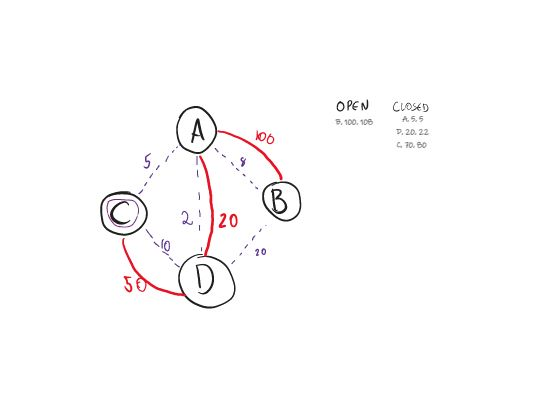
\includegraphics[width=.8\textwidth]{grafo.jpeg}
    \caption{Grafo utilizado para os testes}
    \label{fig:grafo}
\end{figure}

\subsection{Resultados dos testes}\label{sec:res}


\section{Conclusão}\label{sec:concl}

%\bibliography{ref}

\end{document}
